%\documentclass[11pt,a4paper]{report}
\documentclass[11pt,a4paper]{article}
%\documentclass[11pt,a4paper]{amsart}

% 1 inch margins
\usepackage{fullpage}

\usepackage{listings}
  \usepackage{courier}
\usepackage{amsmath}
\usepackage{verbatim}
\usepackage{graphicx}
\usepackage[usenames,dvipsnames]{color}
\usepackage[dvipdf]{hyperref}

\definecolor{codeblock}{rgb}{0.9,0.9,0.9}

\lstset{
language=,
xleftmargin=2em,
%frame=single,
backgroundcolor=\color{codeblock},
basicstyle=\footnotesize\ttfamily,
identifierstyle=\color{Purple},
keywordstyle=\color{OliveGreen},
commentstyle=\color{Red},
stringstyle=\color{RoyalBlue},
showstringspaces=false,
%numbers=left,
%numberstyle=\color{Gray}
}

\lstdefinelanguage{cylctaskdef}
{
morekeywords={NAME,DESCRIPTION,TYPE,CONTACT_DELAY,OWNER,CYCLE_TIMES,EXTERNAL_TASK,ENVIRONMENT,ESTIMATED_RUN_TIME,PREREQUISITES,STARTUP_PREREQUISITES,OUTPUTS,ESTIMATED_RESTART_DUMP_TIMES,SINGLE_CYCLE,ONEOFF_FOLLOW_ON},
sensitive=false,
morecomment=[l]{\#},
morestring=[b]\",
}

\lstdefinelanguage{usage}
{
morekeywords={},
sensitive=false,
morecomment=[l]{Usage:},
morecomment=[l]{Arguments:},
morecomment=[l]{Options:},
morecomment=[l]{Commands:},
morecomment=[l]{usage:},
morecomment=[l]{arguments:},
morecomment=[l]{options:},
morecomment=[l]{commands:},
}


\title{Cylc: A Self-Organising Forecast Systems Scheduler With Optimal
Multi-cycle Catchup Capability}

\author{Hilary Oliver, NIWA}

\begin{document}

\maketitle

\pagebreak
\tableofcontents
\pagebreak

\begin{abstract}

    {\em Cylc} is a self-organising metascheduler\footnote{A
    metascheduler sends dependent tasks to the batch queue job
    scheduler(s) when it has determined that they are {\em ready to
    run}. However, we drop the ``meta'' prefix from here on because a
    metascheduler is also a type of scheduler. The term
    ``metascheduler'' can also refer to a single aggregate view of
    multiple distributed resource managers, but that is not the topic of
    this paper.} for cycling environmental forecast systems consisting
    of any number of linked scientific models and associated data
    processing tasks.\footnote{A {\em task} is any group of processes
    treated as a single entity for scheduling purposes.} Its novel
    scheduling algorithm maintains an evolving pool of task proxy
    objects that interact with each other to resolve all dependencies,
    including those between tasks in different forecast
    cycles.\footnote{For our purposes a {\em forecast cycle} comprises
    all tasks with a common {\em cycle time}, i.e.\ the analysis time or
    nominal start time of a forecast model, or that of the associated
    forecast model(s) for other tasks.} Each task is defined in
    isolation and knows its own prerequisites (but not who will satisfy
    them) and outputs (but not who will use them), and there is no need
    for a global ``suite'' definition that specifies dependencies or
    execution order. Because cylc does not use global time loops to
    advance the system, and treats all dependencies equally, it can run
    tasks from multiple forecast cycles at once to the full extent
    allowed by intercycle dependencies. This matters whenever the
    external driving data\footnote{Forecast systems are typically driven
    by observational data and/or timely model fields from an external
    forecasting system.} for upcoming cycles are available in advance:
    systems can catch up from delays very quickly, parallel test systems
    can be started or restarted behind the main operation to catch up as
    quickly as possible, and historical case studies can achieve
    sustained maximal throughput. In cylc, a series of distinct forecast
    cycles emerges only when and if a system catches up to real time
    operation. Cylc is easily interfaced to existing tasks and is
    extremely flexible and easy to use. It can be restarted in
    arbitrarily complex states of operation and dynamically adapts to
    insertion or removal of tasks in a running system.  Failed tasks
    will necessarily delay their downstream dependants, but the rest of
    the system can carry on unaffected while the problem is addressed,
    after which time the delayed tasks will catch up as quickly as
    possible.  Cylc's handling of forecast model `restart' dependencies
    allows continued operation, with very little operator intervention,
    over major failures that result in omitted forecasts in the driving
    models.  Ability to control the configured task set, and failure
    recovery scenarios, can be completely tested in an accelerated
    simulation mode that is indistinguishable (to cylc) from real
    operation.  Cylc is written in object oriented Python and uses {\em
    Pyro} (Python Remote Objects). It can control tasks across a
    heterogenous distributed network.  

    %\footnote{Cylc also
    %enables new modes of real time operation, for example a catchment
    %river model that runs hourly assimilating real time stream flow
    %observations and using the {\em most recent} 6-hourly precipitation
    %forecast - see EcoConnect, below).} 
\end{abstract}

\pagebreak
\section{How Cylc Works}
\label{sec:FS}

\subsection{Scheduling For Forecast Systems}

Environmental forecasting systems generate forecast products at regular
intervals using potentially large sets of scientific models and
associated data processing tasks. They are constrained by availability
of external driving data, typically real time observations and/or model
data from an external forecasting system, which one or more tasks depend
on, and these drive other ``downstream'' tasks, and so on. The
dependency diagram for such a system consists of one or more (possibly
linked) {\em Directed Acyclic Graphs}, which may vary according to the
{\em forecast cycle} (wherein each task has the same {\em cycle time},
namely the nominal analysis time or start time of the forecast models in
the group). Normal real time operation necessarily consists of a series
of distinct forecast cycles that are each initiated, after a gap in
processing, by arrival of new external driving data.

From a job scheduling perspective task execution order must be carefully
controlled in order to avoid dependency violations. Ideally, each task
should be queued for execution at the instant its last prerequisite is
satisfied; this is the best that can be done even if queued tasks are
not able to execute immediately because of resource contention.


\subsection{An Example: EcoConnect}

This work was motivated by the EcoConnect Forecasting System at NIWA
(National Institute of Water and Atmospheric Research, New Zealand). As
of 2009, EcoConnect takes real time atmospheric and stream flow
observations, and operational global weather forecasts from the Met
Office (UK), and uses these to drive global sea state and regional data
assimilating weather models, which in turn drive regional sea state,
storm surge, and catchment river models, plus tide prediction, and a
large number of associated data collection, quality control,
preprocessing, postprocessing, product generation, and archiving
tasks.\footnote{Future plans for EcoConnect include additional
deterministic regional weather forecasts and a statistical ensemble.}
The global sea state forecast runs once daily.  The regional weather
forecast runs four times daily but it supplies surface pressures to
several downstream models that run only twice daily, and precipitation
accumulations to catchment river models that run on an hourly cycle
assimilating real time stream flow observations and using the most
recent available regional weather forecast.  EcoConnect runs on
heterogenous distributed hardware, including a massively parallel
supercomputer and several Linux servers. 

\subsection{Intracycle Dependencies}

We normally think of dependencies as occuring between tasks within a
forecast cycle. A sea state forecast, for example, might depend on
surface wind fields generated by a weather forecast over the same
forecast range, and a postprocessing task clearly cannot run before its
input data has been generated. Figure~\ref{fig-dep-one} shows the
dependency diagram for a single forecast cycle of a simple example
system consisting of three forecast models ({\em a, b,} and {\em c}) and
three post processing or product generation tasks ({\em d, e} and {\em
f}).  A scheduler capable of handling this must manage, within a single
forecast cycle, multiple parallel streams of execution that branch when
one task generates output for several downstream tasks, and merge when
one task takes input from several upstream tasks. 

\begin{figure} 
    \begin{center}
        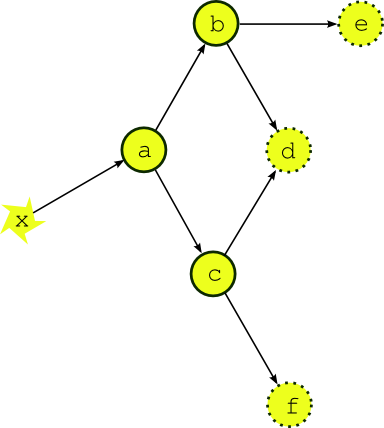
\includegraphics[width=6cm]{inkscape-svg/dep-one-cycle} 
    \end{center}
    \caption{\small Dependency graph for a single forecast cycle of a
    simple example system. Tasks {\em a, b,} and {\em c} represent
    forecast models, {\em d, e} and {\em f} are post processing or
    product generation tasks, and {\em x} represents {\em external
    driving data} that the upstream forecast model depends on.}
    \label{fig-dep-one} 
\end{figure} 

\begin{figure}
    \begin{center}
        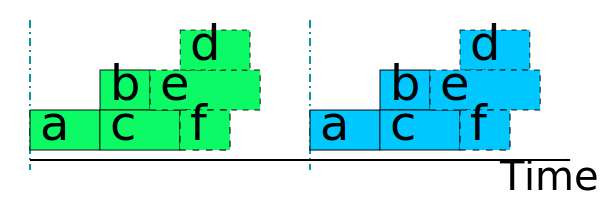
\includegraphics[width=8cm]{inkscape-svg/timeline-one}
    \end{center}
    \caption{\small Job schedule for two consecutive cycles of
the example system during real time operation. The horizontal extent of
each task bar represents its execution time, and the vertical blue lines
show when the external driving data becomes available.}
    \label{fig-time-one}
\end{figure}

Figure~\ref{fig-time-one} shows the job schedule for two consecutive
cycles of the example system in real time operation, given execution
times represented by the horizontal extent of the task bars. There is a
time gap between cycles as the system waits on new external driving
data.  Each task in the example system happens to trigger off upstream
tasks {\em finishing}, rather than some intermediate output or event,
but this is merely a simplification that makes for clearer diagrams.

\begin{figure} 
    \begin{center}
        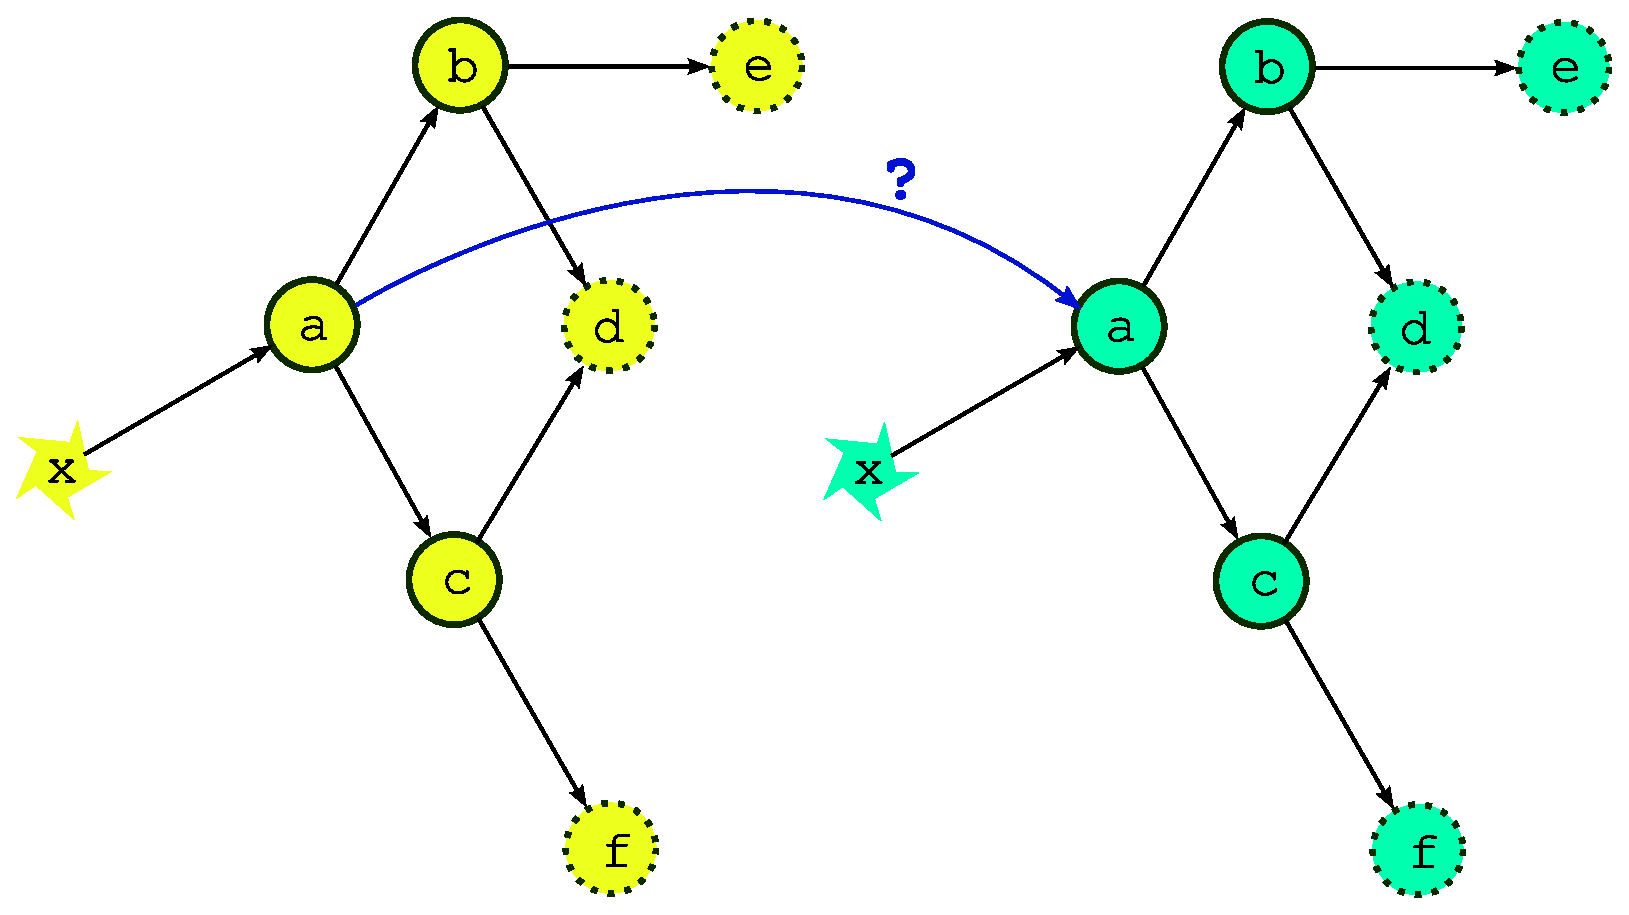
\includegraphics[width=10cm]{inkscape-svg/dep-two-cycles-linked} 
    \end{center}
    \caption{\small If the external driving data is available in
    advance, can we start running the next cycle early?} 
    \label{fig-dep-two-linked}
\end{figure}

\subsection{Intercycle Dependencies}

There are also dependencies between tasks in different cycles: forecast
models typically depend on their own most recent previous forecast for
an initial ``background state'', and different types of tasks in
different forecast cycles can also be linked (e.g.\ the complicated
relationship between the catchment river and weather models in
EcoConnect). In real time operation these intercycle dependencies can be
ignored because they are automatically satisfied when each cycle
necessarily finishes before the next one begins. This is just as well
because they dramatically increase the complexity of the dependency
graph of even the simplest systems, by destroying the clean boundary
between forecast cycles. Figure~\ref{fig-dep-two} illustrates the
problem for our simple example system assuming the least intercycle
dependence likely to be present: the forecast models ($a$, $b$, and $c$)
each depend on their own previous instances.

As far as the author is aware existing schedulers ignore intercycle
dependencies and therefore require a series of distinct forecast cycles
at all times. While this fits with our intuitive view of forecasting
systems, based on normal real time operations, it is a serious
impediment when advance availability of external driving data makes it
possible, in principle, to run some tasks from upcoming cycles before
the current cycle is finished. This occurs after delays (late arrival of
external data, system maintenance, etc.) and, to an even greater extent,
in historical case studies, and parallel test systems that are delayed
with respect to the main operation. It is in fact a serious problem for
systems that have little downtime between forecast cycles and
consequently take many cycles to catch up after a delay. If intercycle
dependencies are ignored the best that can be done, in general, is to
reduce the gap between cycles to zero. A limited crude overlap of the
single cycle job schedule may be possible for specific task sets in
certain circumstances, but this is very much sub-optimal and it would be
difficult to guarantee that dependencies will never be violated.

\begin{figure}
    \begin{center}
        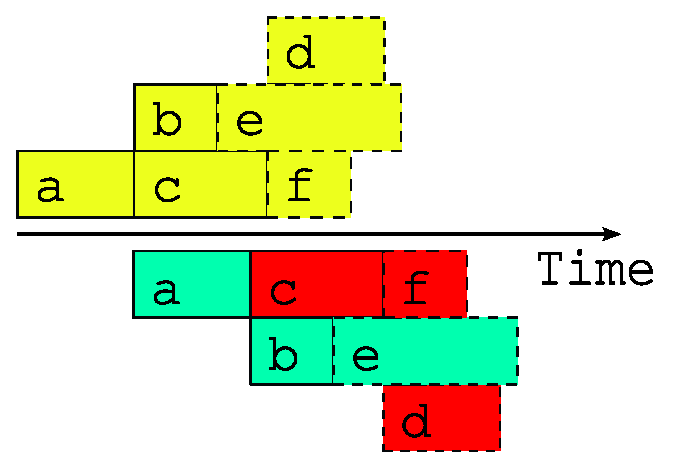
\includegraphics[width=6cm]{inkscape-svg/timeline-one-c} 
    \end{center}
    \caption{\small A naive attempt to overlap two consecutive cycles
    using the single-cycle dependency graph. The red shaded tasks will
    fail because of dependency violations (or will not be able to run
    because of upstream dependency violations).} 
    \label{fig-overlap}
\end{figure} 

\begin{figure}
    \begin{center}
        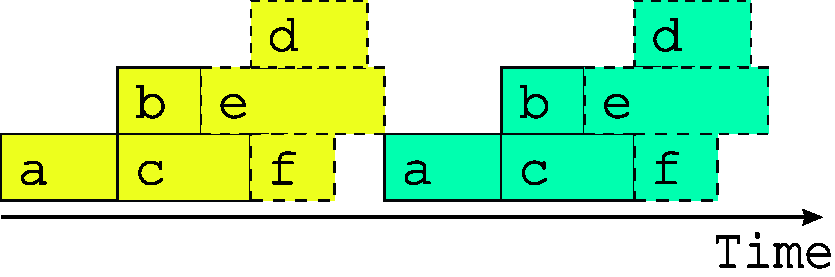
\includegraphics[width=8cm]{inkscape-svg/timeline-one-a} 
    \end{center}
    \caption{\small The best that can be done in general when intercycle dependencies 
    are ignored.} 
    \label{fig-foo}
\end{figure} 

\begin{figure} 
    \begin{center}
        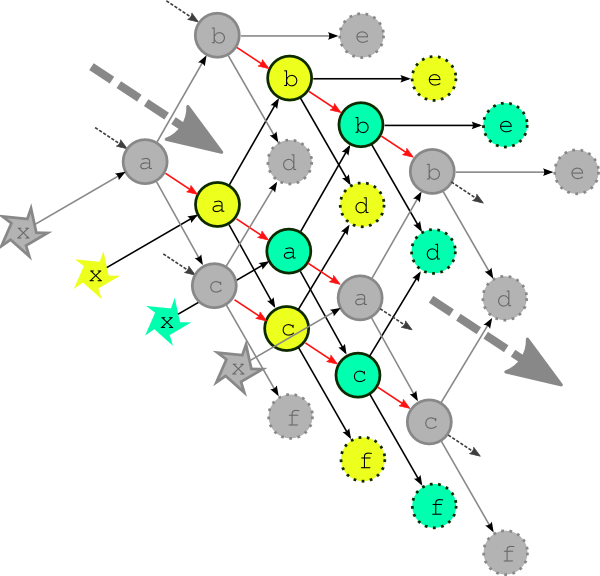
\includegraphics[width=8cm]{inkscape-svg/dep-multi-cycle} 
    \end{center}
    \caption{\small Complete dependency graph for the example
    system, assuming the least possible intercycle dependence: the
    forecast models ($a$, $b$, and $c$) depend on their own previous
    instances. The dashed arrows show connections to previous and
    subsequent forecast cycles.} 
    \label{fig-dep-two}
\end{figure}



Figure~\ref{fig-time-three} shows the effect of an operational delay of
almost one whole cycle on a sequentially cycling system that has little
downtime between cycles - it takes many cycles to catch up. Above the
time axis is the optimal schedule that is possible, in principle, when
intercycle dependencies are taken into account: the second cycle after
the delay is hardly affected, and subsequent cycles are all on time.
Note that simply overlapping the single cycle schedules of 
Figure~\ref{fig-time-one} from the same start point would have resulted in
dependency violation by task {\em c}. Similarly,
Figure~\ref{fig-time-two} shows job schedules for the example system in
case study mode, or when catching up after a very long delay, when the
external driving data are available many cycles in advance.  Task {\em
a}, which as the most upstream forecast model is likely to be a resource
intensive atmosphere or ocean model, has no dependence on cotemporal
tasks and can therefore run continuously, regardless of how much
downstream processing is yet to be completed in its own, or any
previous, forecast cycle. In practice task {\em a} would depend on
cotemporal upstream tasks that wait on the external driving data, but
they would return immediately when the external data is available in
advance, so the result stands. Other tasks can cycle at regular short
intervals, the interval depending on [CHECK THIS] the task run length
relative to that of its longest cotemporal upstream dependency path. In
this case {\em c} can also run continuously, and consecutive instances
of {\em e}, which has no previous-instance dependence, can overlap.
Thus, even for this very simple example system, tasks from three or four
different cycles can in principle run simultaneously at any given
time. 

\subsection{The Cylc Scheduling Algorithm}

\begin{figure} 
    \begin{center} 
        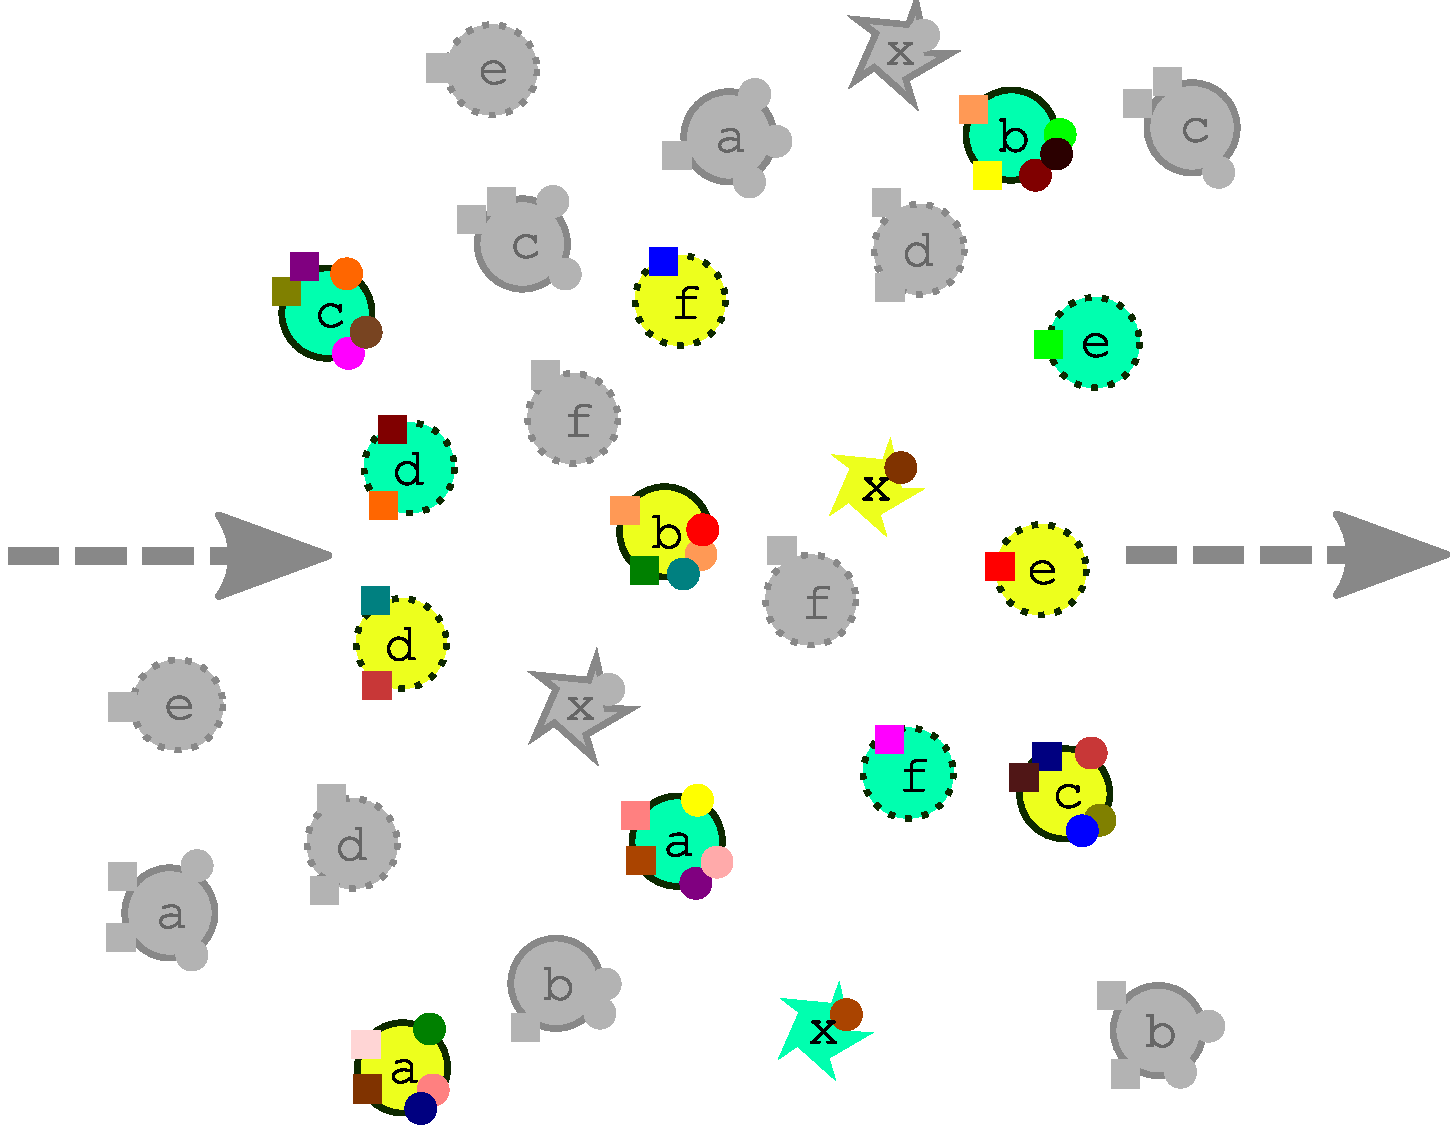
\includegraphics[width=8cm]{inkscape-svg/task-pool}
    \end{center} 
    \caption{\small How cycl sees the task pool, in contrast to the 
    full dependency diagram of Figure~\ref{fig-full}.} 
    \label{fig-time-two}
\end{figure} 

\begin{figure}
    \begin{center}
        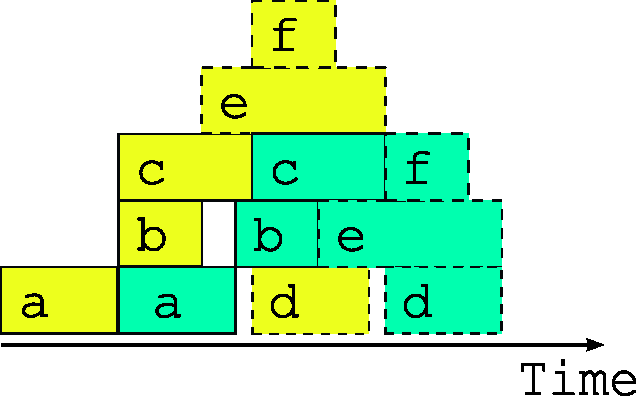
\includegraphics[width=6cm]{inkscape-svg/timeline-two-cycles-optimal} 
    \end{center}
    \caption{\small Optimal job schedule when the next cycle's driving
    data is available in advance, possible in principle when all
    intercycle dependencies are respected.} 
    \label{fig-optimal-two}
\end{figure} 

\begin{figure}
    \begin{center}
        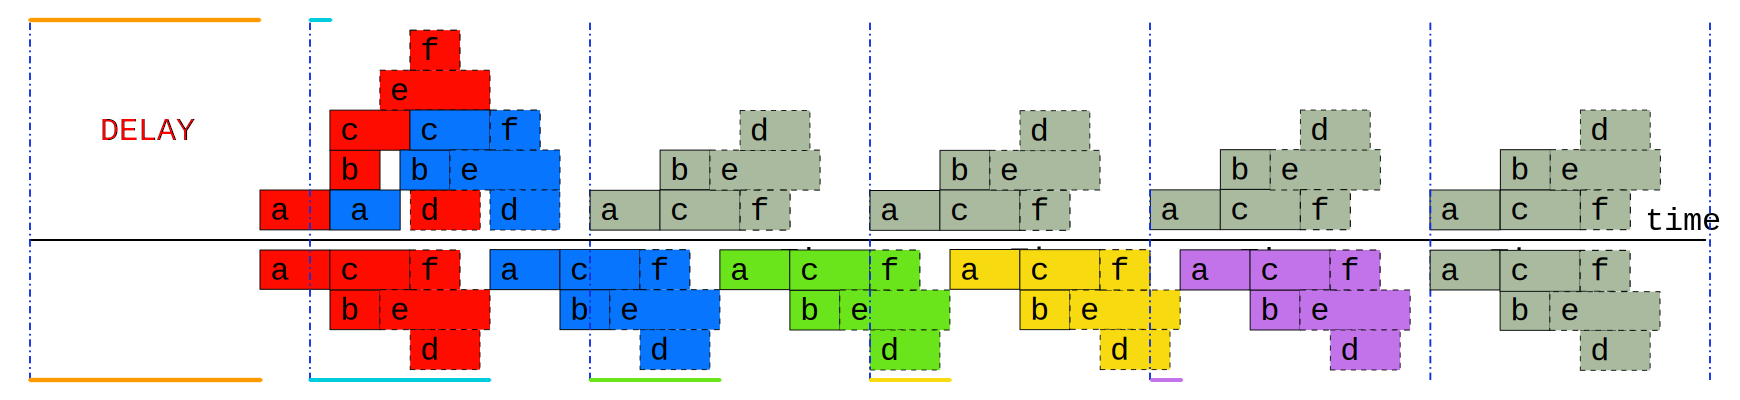
\includegraphics[width=12cm]{inkscape-svg/timeline-three} 
    \end{center}
    \caption{\small Job schedules for the example system after a delay
    of almost one whole forecast cycle, when intercycle dependencies are
    taken into account (above the time axis), and when they are not
    (below the time time axis). The colored lines indicate the time that
    each cycle is delayed, and normal ``caught up'' cycles
    are shaded gray.} 
    \label{fig-time-three}
\end{figure} 

\begin{figure} 
    \begin{center} 
        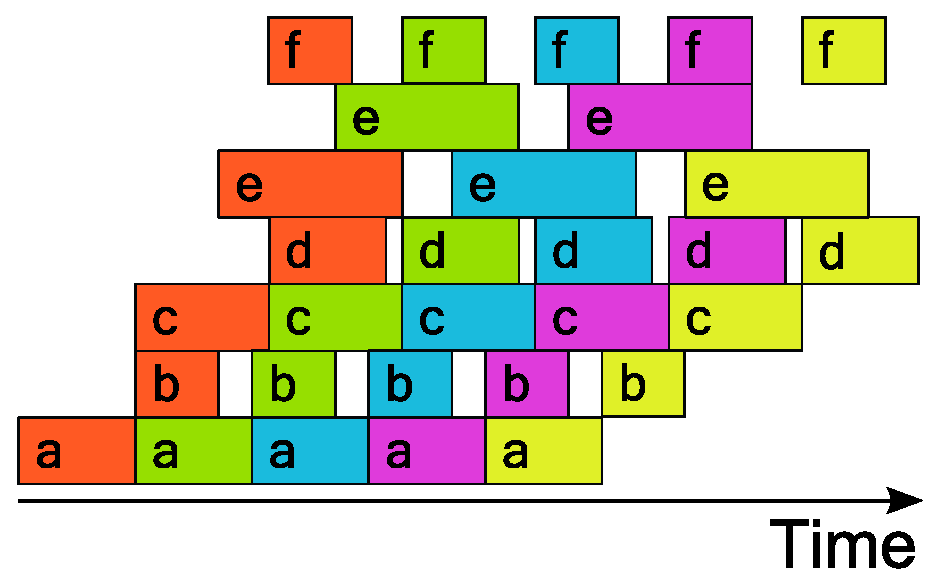
\includegraphics[width=8cm]{inkscape-svg/timeline-two}
    \end{center} 
    \caption{\small Job schedules for the example system in case study
    mode, or after a long delay, when the external driving data are
    available many cycles in advance. Above the time axis is the optimal
    schedule obtained when the system is constrained only by its true
    dependencies, as in Figure \ref{fig-dep-two}, and underneath is
    the best that can be done, in general, when intercycle dependencies
    are ignored.} 
    \label{fig-time-two}
\end{figure} 

Cylc manages a pool of task proxy objects that represent real tasks in
the forecasting system. There is no global cycling mechanism to advance
the system in time; instead each individual task proxy has a private
cycle time and spawns its own successor at the right time (which depends
only on the task's own type and state, not on the state of other tasks
in the system; see Section~\ref{sec:tasktypes}). Task
proxies are self-contained and do not know what other tasks exist in the
system, they just know their own prerequisites and outputs.
Prerequisites can include files (say) that happen to be generated by
other tasks with different cycle times, and the task pool can contain
tasks with many different cycle times.  Now, whenever any task proxy
changes state (as a result of an output completion message, for example)
cylc gets the entire pool to interact indiscriminately, {\em regardless
of cycle times}, in an attempt to match unsatisfied prerequisites with
completed outputs.\footnote{In fact this dependency negotiation goes
through a middleman or broker object, which reduces the task interaction
scaling from $n^2$ to $n$, where $n$ is the number of tasks.} Finally, a
task proxy object can run its real task when its prerequisites are
satisfied and, by means of a messaging system, can record completion of
its own outputs as the system runs. 

Thus without using global cycling mechanisms, and treating all
dependencies equally, cylc in effect gets a set of tasks to
self-schedule by negotiating its own dependencies: optimal scheduling,
as illustrated in the previous section, emerges naturally at run time.
In addition, cylc does not distinguish between delayed and real time
operation at all. In delayed operation the tasks that gather the
system's external driving data will return immediately (because the data
is already available) and the system will only be constrained by its
internal dependencies. In real time operation, the data gathering tasks
will return only when the external data becomes available (normally at
some known time interval after the task's nominal cycle time), delaying
downstream tasks until then, by which time the previous forecast cycle
will have completed. A cylc system thus transitions seamlessly from
optimal multicycle scheduling to ``normal'' distinct forecast cycles as
it catches up to real time operation.

Note that in addition to achieving optimal scheduling, this algorithm is
extremely simple. The operator does not have to specify order of
execution or system dependencies (except implicitly, in that each task's
prerequisites must be matched by someone's outputs). The entire
forecasting system is defined by a simple list of tasks each of which,
in effect, thinks it is alone in the world (even a standalone task must
know its own prerequisites and outputs).\footnote{You can still use
explicit task dependence if you wish: just make a task depend on an
explicitly named upstream supplier {\em finishing} rather than on the
upstream output that is the actual prerequisite of interest. However,
framing prerequisites in terms of required input filenames, or similar,
results in a more flexible system: tasks can easily be ``hot replaced''
by other tasks that generate similar outputs for instance.}  For this to
work, of course, the life cycle of a task proxy object must be such that
it is guaranteed to exist by the time it is needed, but not too much
earlier, and it should die not too long after it is no longer needed.
This requires some thought at the program design stage, but the
complexities therein are entirely hidden from the user. 

\subsection{Comparison with Existing Schedulers}

As explained earlier, as far as the author is aware current forecast
schedulers ignore intercycle dependencies and therefore require
strict sequential cycling, which is very much sub-optimal outside of
normal real time operation. The simplest of these schedulers places the
burden of scheduling almost entirely on the user, who must supply a list
of tasks that the system will run through in order, perhaps with some
way of manually specifying crude functional parallelism.  This is
clearly sub-optimal even for quite simple systems and strict sequential
cycling, and task ordering has to be re-evaluated manually whenever the
system is changed. 

Another approach is hardwired system-specific finite state scheduling
logic that enforces a predetermined order of events: {\em if tasks A and
B have finished, then start task C} and so on. Optimal scheduling within
a forecast cycle is possible in this case, assuming correct coding, but
the hard coded logic inevitably becomes convoluted and inflexible as
system complexity increases, and handling to intercycle dependencies is
almost certainly not feasible.  

Finally, the well established SMS system from ECMWF is an industrial
strength general scheduling tool for dependent jobs. Users define ``SMS
suites'' that group tasks into ``families'' and define explicit
dependency relationships between tasks and/or/? families. SMS does not
appear to be able to do optimal cycle-independent scheduling, however,
or at least is not able to do so when configured for normal usage (THIS
IS STILL NOT ENTIRELY RESOLVED!) because (a) whole families trigger 
at once(?), rather than individual tasks, and global cycling mechanisms
are used to advance the system forward in time (either looping
over successive analysis times for ``catch up'' OR triggering off the
wall clock for real time operation. Thus, in contrast to cylc, it would
not be possible to have a delayed parallel test system catch up to the
main operation and then keep pace with it.

%In other words the task pool must include waiting tasks whose
%prerequisites may {\em soon} be satisfied (but preferably no waiting
%tasks whose prerequisites will not be satisfied for some time yet),
%tasks that are currently running, and finished tasks whose outputs
%could still be needed by any current or future waiting task (but
%preferably not any finished tasks whose output will no longer be needed
%by anyone). 



\pagebreak
\section{Installing Cylc}
\label{sec:usage}

\subsection{System Requirements}

\begin{itemize}
    \item A Unix or Linux operating system
    \item The Python programming language
    \item Pyro (Python Remote Objects)
\end{itemize}

Cylc has been tested with Python 2.4.2 and 2.6.x, and Pyro 3.9 and 3.10,
but it should work well with any recent versions or Python 2 and Pyro.
As yet Pyro is not compatible with Python 3.  Download Pyro from {\em
http://pyro.sourceforge.net}, and follow its simple installation
instructions (it installs in the standard Python modules path).


\subsection{Installation}

Cylc is currently maintained using {\em darcs}, a distributed revision
control system. If you need to develop cylc you can request access to
clone the central repository, otherwise you will receive a cylc
distribution tarball. Cylc is designed to be installed into a directory
under a normal user account: simply unpack the tarball. There is no
``build'' required because cylc is written in Python (and a few small 
bash scripts).

After installing cylc, modify your login environment to get access to
the bin directory and Python source modules. For bash or ksh login
shells, for example, add the following to \lstinline=$HOME/.profile= 

\lstset{language=bash} 

\begin{lstlisting}
    # provide access to the cylc scheduler
    CYLC=#INSERT-PATH-TO-TOP-LEVEL-CYLC-INSTALLATION-DIR
    export PATH=$CYLC/bin:$PATH
    export PYTHONPATH=$CYLC/src:$PYTHONPATH
\end{lstlisting}

\subsection{Testing}

Test the new installation by running the packaged example systems
(Section~\ref{sec:examples}). These should work ``out of the box'', but
refer to the rest of this document, and/or \lstinline=cylc help= for
more information.  

First configure the system (only required the first time, and after
changing the system's task set) and start scheduling it with cylc:

\begin{lstlisting}
    # configure the simple-0 system
    cylc configure --system simple-0 $CYLC/sys/examples/simple-0
    # start scheduling in dummy mode
    cylc schedule --system simple-0 --dummy-mode 2010081012
\end{lstlisting}

In another terminal window open a monitor to view the running system:

\begin{lstlisting}
    # monitor the running system
    cylc monitor --system simple-0 -a
\end{lstlisting}

In yet another terminal, shut the system down by remote control:

\begin{lstlisting}
    # shut the system down
    cylc control --system simple-0 --stop
\end{lstlisting}

Finally, rerun the system for real (omit the \lstinline{--dummy-mode}
option above).

\pagebreak
\section{Quick Start Guide}

The following is a quick summary of the steps required to get a system
running under cylc.

\subsection{Define The System}

\begin{itemize}
    \item divide your system into {\bf tasks} with clearly defined 
        {\bf prerequisites} and {\bf outputs} (Section~\ref{sec:tasks}).

    \item write a {\bf task definition file} for each task
        (Section~\ref{sec:taskdefs}).

    \item write {\bf task scripts} to run the real external tasks 
        (Section~\ref{sec:taskscripts}).

\end{itemize}

\subsection{(Re)Configuring A System}

Tell cylc to generate a task class module and config file for the new
system (Section~\ref{sec:configure}): 

\begin{lstlisting}
    cylc configure --system SYSTEM [options]
\end{lstlisting}

This must be done whenever system tasks are added, removed, or modified.
Customise the config file if necessary.

\subsection{Running A Configured System}

To cold start or restart a configured system (Section~\ref{sec:run}):

\begin{lstlisting}
    cycl schedule --system SYSTEM [options]
\end{lstlisting}
    
\subsection{Monitoring A Running System}

Use one or more of the terminal based cylc system monitors
(Section~\ref{sec:monitor}). For the main monitor: 

\begin{lstlisting}
    cylc monitor --system SYSTEM [options]
\end{lstlisting}

\subsection{Controlling A Running System}

To interrogate, add or delete tasks, shutdown, etc. (Section~\ref{sec:control}):

\begin{lstlisting}
    cylc control --system SYSTEM [options]
\end{lstlisting}


\subsection{General Guidelines}

Build and test your system incrementally using {\bf dummy mode}
(Section~\ref{sec:dummymode}).


\pagebreak
\label{sec:tasktype}
\section{Defining Tasks}

First divide your system into tasks of known {\bf type}, with clearly
defined {\bf prerequisites} and {\bf outputs}.

\label{sec:tasktype}
\subsection{Task Type}

In other scheduling systems, as explained earlier, groups of tasks with
the same cycle time must complete before a new batch of tasks, at the
next cycle time, is ready to run. In cylc, each task propagates itself
forward in time by spawning its own successor, at the next cycle time 
valid for that task, at the right time. When this occurs depends on the
type of task. 

\begin{itemize}
    \item \lstinline=free_task= - this task type does not depend on
        previous instances of itself at all, so it can spawn its
        successor as soon as it enters the 'running'
        state\footnote{A free task could potentially spawn before
        entering the 'running' state, but this would have no further
        advantage in terms of parallel execution at a cost of
        unrestrained breeding EXPLAIN BETTER} earlier than
        i.e.\ multiple instances of a free task can run simultaneously,
        or at least overlap in time, if the opportunity arises (which
        depends on its prerequisites). Most non-forecast model tasks
        (pre and post processing tasks, etc.) should be of this type
        (but see the 'sequential' modifier below).    

    \item \lstinline=forecast_model= - 
\end{itemize}


\label{sec:requisites}
\subsection{Prerequisites and Outputs}


\pagebreak
\label{sec:taskdef}
\subsection{Task Definition Files}

A task definition file declares the properties of each task in a simple
text format.  \lstinline=cylc configure= parses a system's task definition
files uses the information declared therein to generate (i) a Python
task class module, and (ii) a config file, for the system.

The following listing shows an example task defintion represents a
typical non-forecast-model task. The vast majority of tasks in any
typical system would not be any more complicated than this, but see the
task definition reference (Section~\ref{sec:taskdefref}) for the full
range of options available.

\lstset{language=cylctaskdef}

{
\lstinputlisting{../sys/templates/example-task.def}
}

\pagebreak
\subsection{Task Scripts}

(note that several tasks may use the same script with different
arguments, e.g. for moving files around).

\subsection{Task Messaging}

Each external task must:

\begin{itemize}
\item report (to cylc) when the task has started
\item report when the task has finished
\item report when every other registered task output has
completed
\end{itemize}

(Technically, the `started' and `finished' messages are just
outputs too, but they are special in that every task
must have them).

In addition, tasks can optionally:

\begin{itemize}
\item report any arbitrary unregistered (i.e. non-output)
messages, for debugging, logging, or progress monitoring purposes.
\end{itemize}

All incoming messages are logged by cylc, but only output messages can
affect the state of other task objects.

Task messages don't necessarily have to originate from top level task
control scripts. It's a probably a good idea to do this if possible, but
lower level scripts that are invoked as the task runs can communicate
directly with cylc if necessary.

\subsection{Task Wrapping}

A simple a simple wrapper script invoked by cylc reports task
startup, invokes the task, and reports task completion or failure. 

\pagebreak
\section{Configuring A System}

\subsection{System Config Files}

Each task set to be scheduled by cylc requires a {\bf config file} that
specifies system-dependent parameters such as name, list of tasks to
run, logging directory path, and so on. The config file is generated
automatically by \lstinline=cylc configure= the first time the system's
task definition files are parsed. Subsequent reconfiguration will not
overwrite the config file unless you force it (in which case the
original will be backed up), in case you have changed the default
settings. The config file is a Python source module, but it is simply
structured and should be easy for non-programmers to understand. 

All configurable items are stored in a single {\em dict} (a Python
associative array):

\lstset{language=Python}
\begin{lstlisting}
config[ 'item' ] = value
\end{lstlisting}

\subsection{Configurable Items}

\begin{itemize} \item {\bf system name}: the system is registered under
        this name in your cylc preferences directory. The system name is
        then used to refer to the system in cylc commands. It is also
        used as a ``groupname'' under which to register system objects 
        in the Pyro nameserver, to prevent conflicts with other systems
        that may be running at the same time.

        \begin{lstlisting}
config['system_name'] = 'foo'
        \end{lstlisting}

    \item {\bf task list}: list the name of each task to instantiate at
        system startup.  For testing and debugging you can turn off
        specific tasks by simply commenting them out of the task list.
        
        \begin{lstlisting}
config['task_list'] = \
    [
        'foo',
        #'bar',
        'baz'
    ]
        \end{lstlisting}


    \item {\bf task groups}: you can group several related tasks under a
        single name for easy dynamic insertion of multiple tasks at
        once into a running system. For example, you could define a 
        group to hold all the tasks needed to cold start a particular
        model.

        \begin{lstlisting}
config['task_groups']['foo'] = [ 'bar', 'baz', ...]
        \end{lstlisting}

    \item {\bf job launch method}: the method by which cylc should
        invoke the real external tasks when their prerequisites are
        satisfied. Current methods are
        \begin{itemize}
            \item {\bf qsub}: sudo submit to a named queue as the task
                owner.  
            \item {\bf not qsub}: direct background execution.
        \end{itemize}
        To add additional external launch methods (e.g.\ for other
        queueing systems) you will need to modify the 
        \lstinline{src/task_launcher.py} source module.

        \begin{lstlisting}
config['use_qsub'] = True
config['job_queue'] = 'prime'
        \end{lstlisting}

    \item {\bf state dump directory}: the location of cylc's ``state
        dump'' files (see Section~\ref{sec:state-dump}).  You may
        specify an absolute directory path, or one relative to the
        directory in which you run cylc.
        
        \begin{lstlisting}
config['logging_dir'] = '/foo/bar/baz/state'
        \end{lstlisting}


    \item {\bf logging directory location}: 
        This items sets the location of the system's log files. You may
        specify an absolute directory path, or one relative to the
        directory in which you run cylc.

        \begin{lstlisting}
config['logging_dir'] = '/foo/bar/baz/logging'
        \end{lstlisting}

    \item {\bf logging verbosity}: Cylc's logging subsystem is based on
        the standard Python logging module (see
        Section~\ref{sec:logging}). The 'info' level logs messages
        relevant to task execution and scheduling, while the more
        verbose 'debug' level adds messages that trace the execution of
        cylc itself.

        \begin{lstlisting}
config['logging_level'] = logging.INFO
        \end{lstlisting}

    \item {\bf environment variables}: You can export variables into the 
        environment of all external tasks that the system runs. Note that
        this can also be done, via task definition files, on a per-task
        basis.

        \begin{lstlisting}
config['environment'] = {'VAR1':'value1', 'VAR2':'value2', ... }
        \end{lstlisting}

    \item {\bf global system constraint}: if your system contains a
        subset of tasks that do not depend on other tasks in the system, 
        you can prevent these tasks from running out far ahead of the 
        rest by setting the maximum interval (with respect to cycle
        time) that the fast task is allowed to get ahead of the slowest.
        
        \begin{lstlisting}
config['max_runahead_hours'] = 24
        \end{lstlisting}

\end{itemize}


\pagebreak

\subsection{An Example Config File}

This is the config file for the ``simple-0'' example system distributed
with cylc: 

\lstset{ language=Python }
{
\lstinputlisting{../sys/examples/simple-0/system_config.py}
}

\pagebreak

\lstset{language=}

\pagebreak
\section{Running Cylc}

\label{sec:dummymode}
\subsection{Dummy Mode}

In {\em dummy mode}, \lstinline=cylc schedule -d=, in place of each real
system task cylc executes an external program that masquerades as the
real task by reporting its registered outputs complete at the appropriate
times. This is essentially indistinguishable, to cylc, from the real
thing, and is therefore a complete test of scheduling for the configured
task set. Dummy mode allows very quick testing of scheduling and failure
recovery scenarios for arbitrarily complicated task sets.


\section{System Monitors}

\section{Interacting With Running Systems}

\section{Packaged Example Systems}

\pagebreak
\section{Command Reference}


All cylc commands are self documenting, so this section is
auto-generated during document processing.

\subsection{cylc}

\lstset{language=usage}

This is the command line interface to all cylc commands.

{
\lstinputlisting{command-usage/cylc.txt}
}

\pagebreak
\subsection{cylc configure}

Run this command whenever a system's task definition files have been
modified. It generates a Python task class module for the system, and a
default config file that can be customized by the user, and it registers
the configured system by name under your cylc preferences directory
(\lstinline=.cylc/=).

{ 
\lstinputlisting{command-usage/cylc-configure.txt} 
}

\pagebreak
\subsection{cylc schedule}

This is the scheduler program itself. You can run multiple scheduler
instances at once (e.g.\ to control a main operation and several
parallel test systems) so long as each system is configured with a
different name. 
{
\lstinputlisting{command-usage/cylc-scheduler.txt}
}

\pagebreak
\subsection{cylc control}

Use this command to interact with (interrogate and control) running systems.

{
\lstinputlisting{command-usage/cylc-controller.txt}
}

\pagebreak
\subsection{cylc monitor}
{
\lstinputlisting{command-usage/monitor.txt}
}

\subsection{cylc monitor-r}
{
\lstinputlisting{command-usage/monitor-r.txt}
}

\subsection{cylc monitor-d}
{
\lstinputlisting{command-usage/monitor-d.txt}
}

\subsection{cylc monitor-p}
{
\lstinputlisting{command-usage/monitor-p.txt}
}

\pagebreak
\section{Task Definition Reference}

A {\em Task Definition File} defines the properties of a cylc task:
name, valid cycle times, prerequisites and outputs, the task
control script used to invoke the external task, etc.  
\lstinline=cylc configure= parses a system's task definition files and
generates the Python task class module required by cylc to run the
system.

Listed below is the full task definitition template with all items documented.

\lstset{language=cylctaskdef}

{
\lstinputlisting{../sys/templates/full-template.def}
}

\lstset{language=}

%\pagebreak
%\subsection{More Complex Task Behaviour}

%DETAIL WHEN IS IT NECESSARY TO DERIVE PYTHON TASK CLASSES DIRECTLY
%I.E. WHEN ARE CYLC TASK DEFINITION FILES NOT SUFFICIENT.
%(In EcoConnect: only streamflow and topnet)

\pagebreak
\appendix

\section{Object Oriented Programming}

Cylc relies heavily on Object Oriented Programming (OOP) concepts,
particularly the {\em polymorphic} nature of the task proxy objects.
This section gives a very minimal explanation of what this means;
please refer to an OOP reference for more detail.

A {\bf class} is a generalisation of data type to include behaviour
(i.e.\ functions or methods) as well as state. 

%For example, a $shape$ class could define a $position$ data member to
%hold the location of a shape object, a $move()$ method that by which
%a shape object can alter its position, and a $draw()$ method that
%causes it to display itself on screen.

An {\bf object} is a more or less self contained specific instance
of a class. This is analagous to specific integer variables being 
instances of the integer data type.

A {\bf derived class} or {\bf subclass} {\em inherits} the properties
(methods and data members) of its parent class. It can also override
specific properties, or add new properties that aren't present in the
parent. Calling a particular method on an object invokes the object's
own method if one is defined, otherwise the parent class is searched,
and so on down to the root of the inheritance graph. 

%For example, we could derive a $circle$ class from $shape$, adding a
%`radius' data member and overriding the $draw()$ to get circle objects
%to display themselves as actual circles.  Because we didn't override the
%$move()$ method, calling $circle.move()$ would invoke the base class
%method, $shape.move()$. 


{\bf Polymorphism} is the ability of one type to appear as and be used
like another type.  In OOP languages with inheritance, this usually
refers to the ability to treat derived/sub-class objects as if they were
members of a common base class. In particular, a group of mixed-type
objects can all be treated as members of a common base class. 
%For example, a group of %$circles$, $triangles$, and $squares$ could 
%be manipulated by code designed entirely to handel $shapes$; calling
%$[shape].draw()$ will invoke the right derived class $draw()$ method. 
This is a powerful mechanism because it allows an existing program,
without modification, to manipulate new objects so long as they 
derive from the same base class as the original objects.
%If we later derive an entirely new kind of shape ($hexagon$, say) with
%it's own unique behaviour, the existing program, without modification,
%will process the new objects in the proper hexagon-specific way.  

In cylc, all task proxy objects are derived from a base class that 
embodies the properties and behaviour common to all task proxies. 
The scheduling algorithm works with instances of the base class so that
any current or future derived task object can be handled by the program
without modification (other than deriving the new subclass itself).


\pagebreak
\section{Threading in Pyro} \label{pyro-appendix}

In single threaded mode Pyro's \lstinline=handleRequests()= returns
after either a timeout has occurred or at least one request
(i.e.\ remote method call) was handled. Using \lstinline|timeout = None| 
allows us to process tasks {\em only} after remote method invocations
come in.  Further, we can detect the remote calls that actually change
task states, and thereby drop into the task processing code only when
necessary, which eliminates a lot of extraneous output when debugging
the task processing loop (e.g.\ in dummy mode there are a lot of remote
calls on the dummy clock object, which does not alter tasks at all). 

In multithreaded mode, \lstinline=handleRequests()= returns immediately
after creating a new request handling thread for a single remote object,
and thereafter remote method calls on that object come in asynchronously
in the dedicated thread. This is not good for cylc's scheduling
algorithm because tasks are only set running in the task processing
block which can be delayed while \lstinline=handleRequests()= blocks waiting
for a new connection to be established, even as messages that warrant
task processing are coming in on existing connections. The only way
around this seems to be to do task processing on \lstinline=handleRequests()=
timeouts which results in a lot of unnecessary processing when nothing
important is happening.


\pagebreak
\section{Miscellaneous Notes}

\subsection{Orderly Product Generation}

Note that ``correct scheduling'' is not equivalent to ``orderly
generation of products by cycle time'' - under cylc a product
generation task will trigger as soon as its prerequisites are satisfied,
whether or not other tasks associated with the same cycle time are
running yet. If your product presentation or delivery system demands
that all products for one cycle are complete before any from the next
cycle, then (a) this is inefficient - fix it!, or (b) introduce artificial
dependencies into your system to enforce strict sequential cycling (but
that, of course, nullifies the principal advantage of using cylc in the
first place!), or (c) write a script that monitors the output from 
your cylc system and reports completion of a cycle only when the last
products associated with that cycle are complete. 

%\subsection{Catching Up}
%
%The state of being ``caught up'' or not is a property of individual
%tasks, not the whole system, and additionally it should only matter to
%external contact tasks, i.e. those that wait on external data that is
%available at a wall clock time of T (task cycle time) + o (some offset
%insterval). Where this matters an external task can detect whether or
%not it has caught up (and signal this to its proxy object in cylc) by
%comparing its cycle time (and offset) to the wall clock time.

\end{document}
